\documentclass[final]{beamer}

% ====================
% Packages
% ====================

\usepackage[T1]{fontenc}
 \usepackage[utf8]{luainputenc}
\usepackage{lmodern}
\usepackage[size=custom, width=120,height=90, scale=1.2]{beamerposter}
\usetheme{gemini}
\usecolortheme{cam}
\usepackage{graphicx}
\usepackage{booktabs}
\usepackage{tikz}
\usepackage{pgfplots}
\pgfplotsset{compat=1.14}
\usepackage{anyfontsize}
\usepackage{fontawesome5}
\usepackage{algorithm}
\usepackage{algpseudocode}
\usepackage[backend=biber,style=ieee]{biblatex}

\addbibresource{references.bib}

\graphicspath{{../figures/}}

% ====================
% Lengths
% ====================

% If you have N columns, choose \sepwidth and \colwidth such that
% (N+1)*\sepwidth + N*\colwidth = \paperwidth
\newlength{\sepwidth}
\newlength{\colwidth}
\setlength{\sepwidth}{0.025\paperwidth}
\setlength{\colwidth}{0.3\paperwidth}

\newcommand{\separatorcolumn}{\begin{column}{\sepwidth}\end{column}}
\renewcommand*{\bibfont}{\footnotesize}


% ====================
% Title
% ====================

\title{Practical Analysis of Hybrid Sorting Algorithms}

\author{Joshua Arulsamy}

\institute[shortinst]{Department of Electrical Engineering and Computer Science, University of Wyoming}

% ====================
% Footer (optional)
% ====================

\footercontent{
  \faGithub\ \href{https://github.com/uwyo-mallet/Hybrid-Sorting-Optimization}{https://github.com/uwyo-mallet/Hybrid-Sorting-Optimization} \hfill
  Undergraduate Research and Inquiry Day 2023 \hfill \hfill
  \href{mailto:jarulsam@uwyo.edu}{jarulsam@uwyo.edu}
}
% (can be left out to remove footer)

% ====================
% Logo (optional)
% ====================

% use this to include logos on the left and/or right side of the header:
% Left: institution
 \logoleft{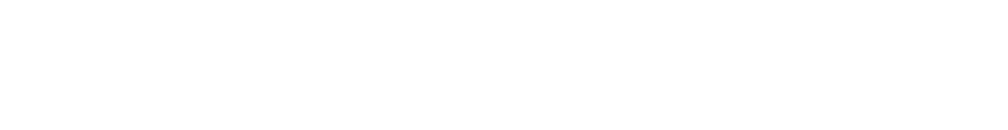
\includegraphics[height=3.0cm]{logos/New_UWSignature_1_line_White_Web.png}}
% Right: funding agencies and other affilations
% \logoright{
\includegraphics[height=2.5cm]{logos/WRSP/abbreviated/UWabbreviated_V_WRSP_white.png}}
% ====================
% Body
% ====================

\begin{document}

\addtobeamertemplate{block begin}{\vskip -\bigskipamount}{}
\addtobeamertemplate{block end}{}{\vskip -\bigskipamount}

\begin{frame}[t]
	\begin{columns}[t]
		\separatorcolumn

		\begin{column}{\colwidth}

			\begin{block}{Introduction}
				\begin{itemize}
					\item Most applications require data to be arranged in a certain order.
					      The procedure of reordering data according to some comparator is
					      called sorting. Sorting can be found in nearly every computer
					      system today.
					\item The near omnipresent need for
					      performant sorting implementations has resulted in most major
					      programming languages including a type-generic sorting function
					      within their standard libraries.
					\item This research analyzes a wide variety of sorting
					      algorithm implementations across varying system architectures to
					      determine optimal parameter configurations for hybrid sorting
					      algorithms.
					\item This research also proposes a new performant standard
					      sorting implementation for GNU's C standard library
					      leveraging, Mergesort, insertion sort, and sorting
					      networks.
				\end{itemize}
			\end{block}

			\begin{block}{Background}
				\begin{itemize}
					\item Substantial effort has been spent on the analysis of
					      sorting algorithms. Typically, two major characteristics
					      are considered when studying sorting algorithms; space
					      and time complexity\parencite{Bentley1993EngineeringAS}.
					\item Existing analysis of popular sorting algorithms, such as Quicksort
					      and Mergesort, place substantial emphasis on their excellent
					      asymptotic complexity in the average case\parencite{glibc}.
					\item Asymptotic complexity alone does not describe the
					      practical performance of these algorithms. While Mergesort may
					      have a better asymptotic time complexity in the worst case than
					      insertion sort, for small inputs, insertion sort typically
					      outperforms Mergesort by avoiding the overhead of recursive calls.
				\end{itemize}
			\end{block}

			\begin{block}{Proposed Algorithms}
				\begin{itemize}
					\item The proposed algorithm is a highly-optimized version of
					      Mergesort leveraging both insertion sort and a network
					      sorting algorithm.
					\item During recursive calls of conventional Mergesort, if the
					      subarray's length is less than a threshold value,
					      insertion sort is used instead.
					\item In instances where a subarray contains less than 5
					      elements, a comparison-optimal network sorting algorithm
					      is used instead.
				\end{itemize}
			\end{block}

			\begin{block}{Experimental Setup}

				A small subset of algorithms is chosen for evaluation. Primarily,
				algorithms utilized within standard library implementations are of
				particular interest, since they are typically highly performant in
				the general case. Other complementary algorithms which perform
				exceptionally well in specific scenarios are also evaluated. Since
				this analysis is focused on analyzing and improving existing
				implementations, general purpose sorting function are taken from
				various standard libraries, such as GNU's libc\parencite{glibc}
				and musl libc\parencite{musl_libc}.

				\begin{enumerate}
					\item \textbf{Each algorithm is timed while sorting the same
						      data using a variety of threshold values.} This is
					      repeated 1,000 times. The mean is calculated for each
					      algorithm. This is done to minimize noise (time
					      inaccuracy, other processes on the test system, etc.)
					      during data collection.
					\item \textbf{Each algorithm configuration is tested on a
						      variety of platforms}. To determine whether the
					      algorithms perform well across a variety of
					      architectures, each test is repeated on different,
					      commonly used systems.
					\item \textbf{Results are examined}. The performance
					      differences from the standard built-in sorting function
					      \texttt{qsort} are calculated and plotted. This function
					      serves as a baseline to compare performance against.
				\end{enumerate}
			\end{block}
		\end{column}

		\separatorcolumn

		\begin{column}{\colwidth}

			\begin{block}{Results}
				The proposed algorithm (Mergesort w/ Fast InsSort \& Network)
				outperforms all other evaluated algorithms in most scenarios. Most
				notably, entirely random data (Fig. \ref{fig:random}) see's an
				upward of 15\% runtime reduction. Pipe organ data (Ex. 1, 2, 3, 4,
				3, 2, 1) (Fig. \ref{fig:pipeorgan}) saw significant improvement in
				performance as well at nearly a quarter the runtime of the
				existing \texttt{qsort} implementation.

				\begin{figure}[h]
					\centering
					\makebox[\colwidth]{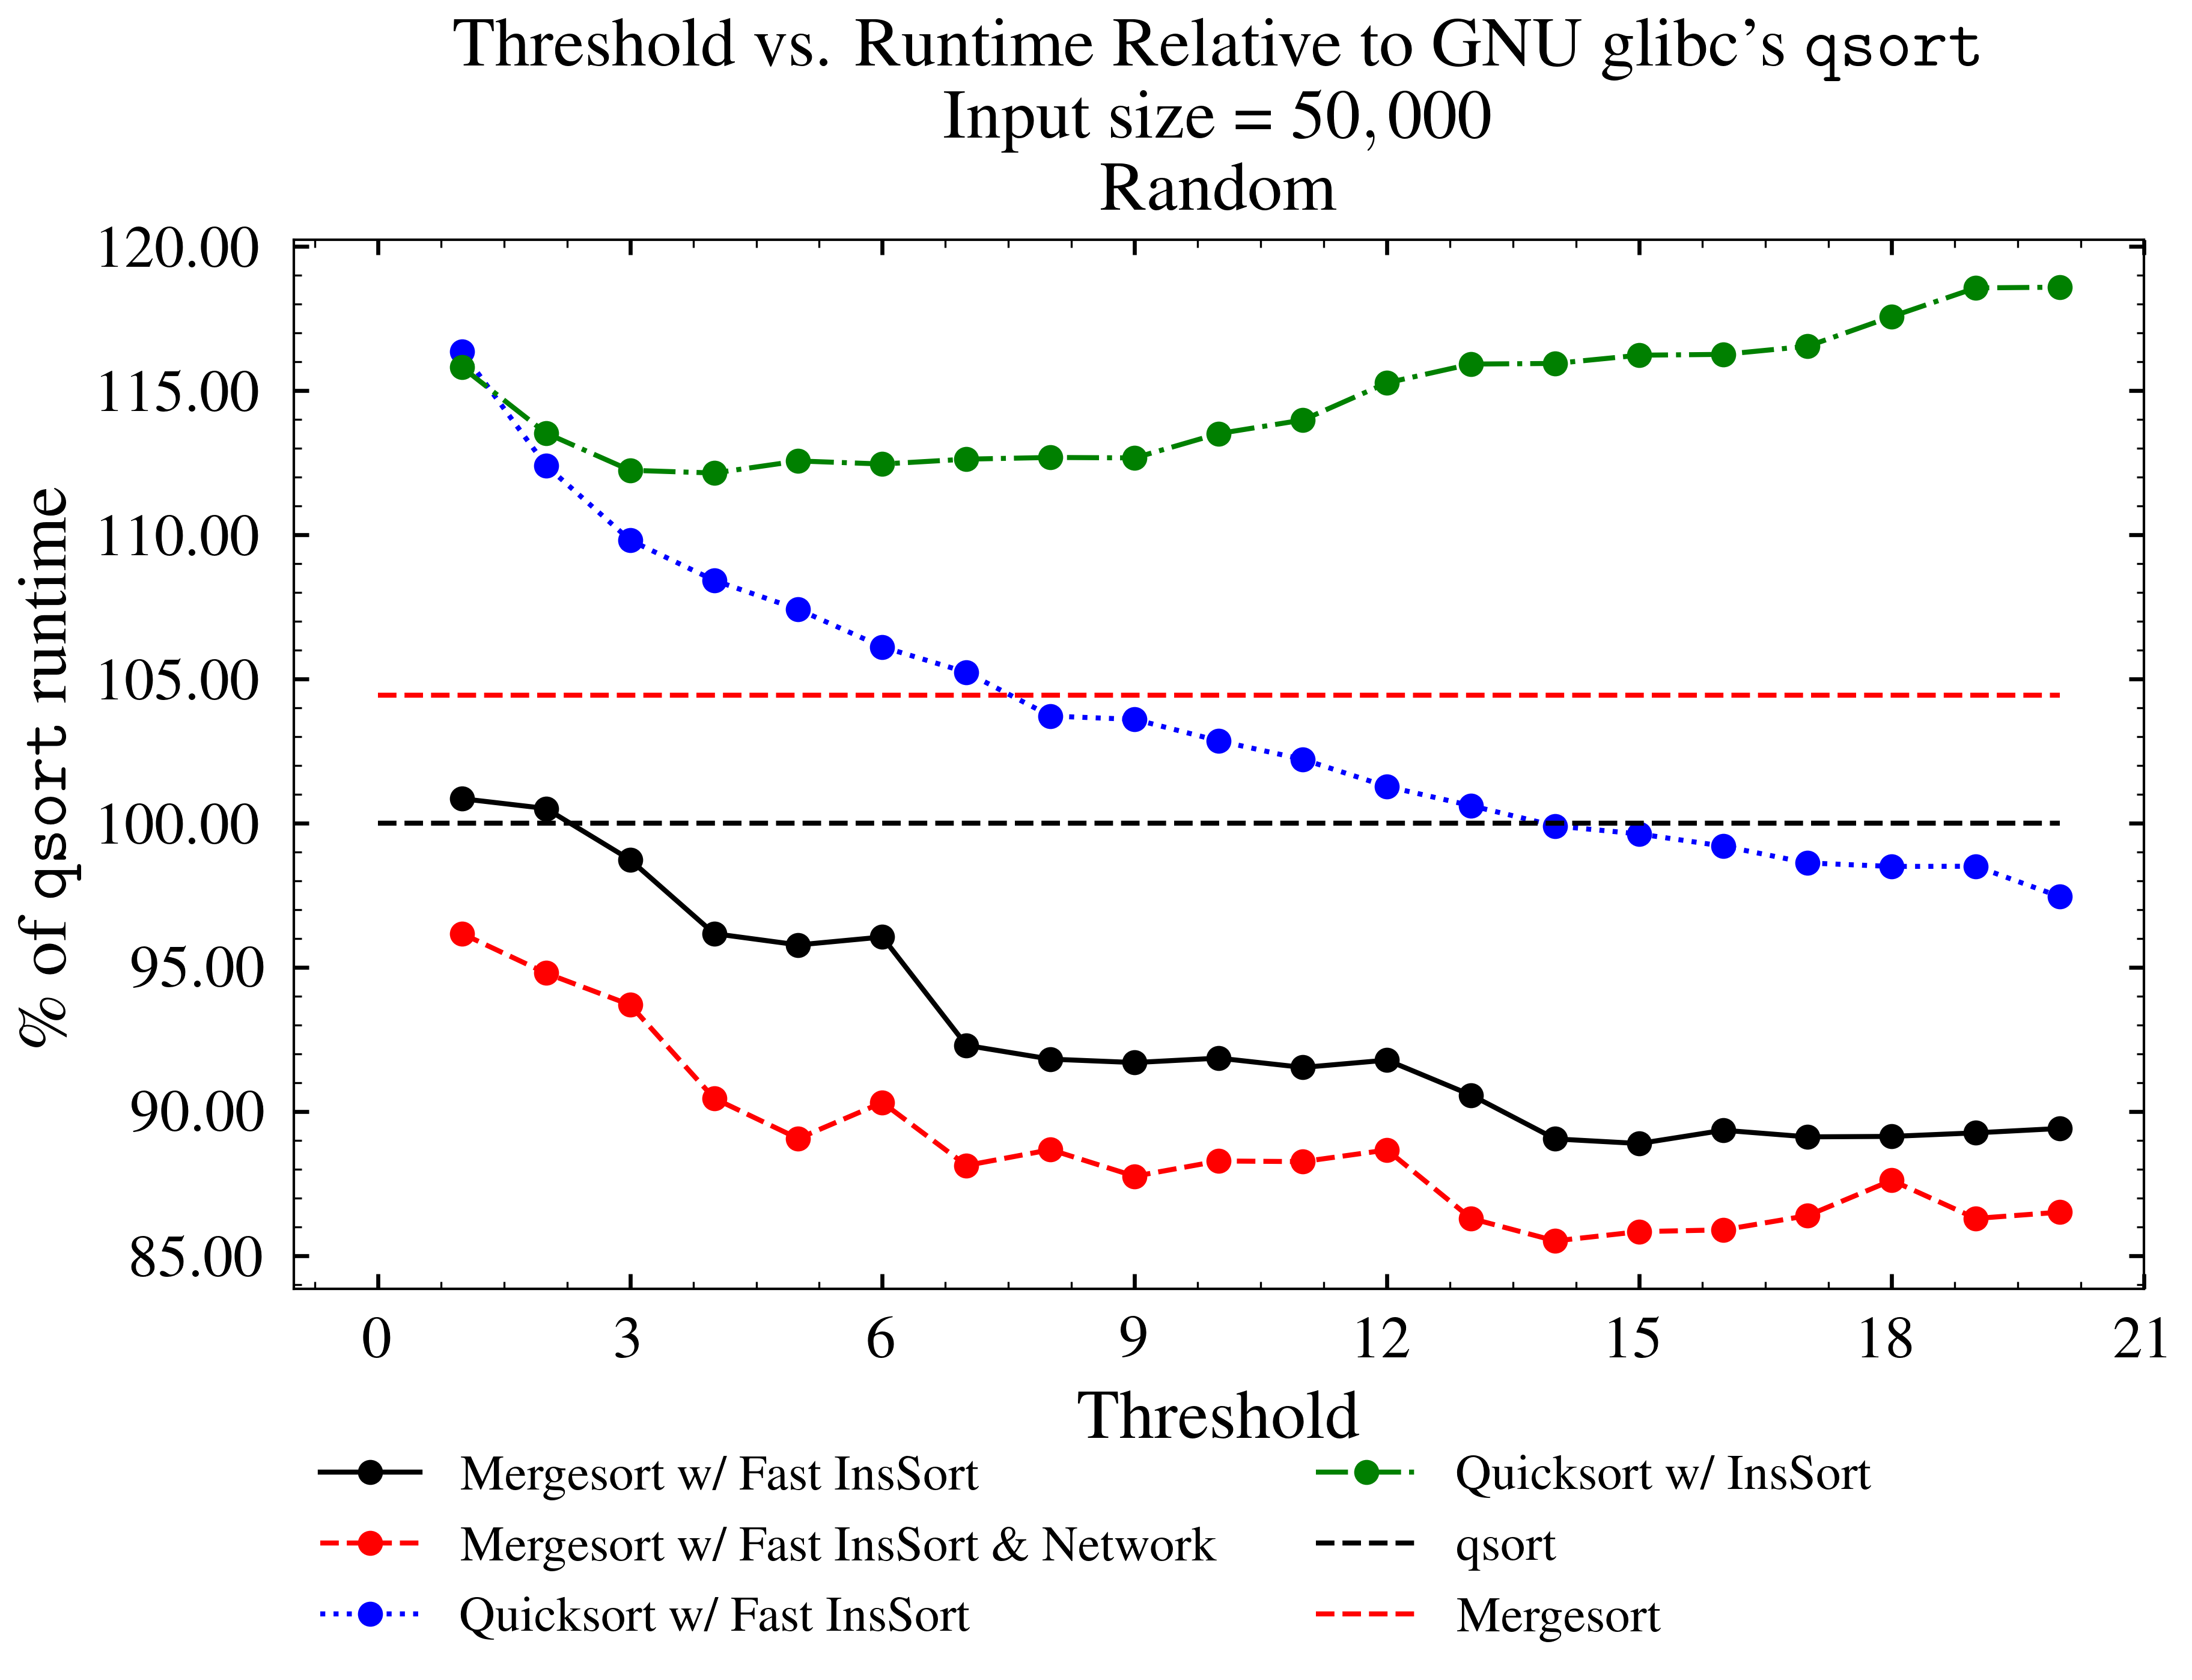
\includegraphics[width=\colwidth]{random}}
					\caption{Runtime vs. Threshold on Random Input Data}
					\label{fig:random}
				\end{figure}
				\begin{figure}[h]
					\centering
					\makebox[\colwidth]{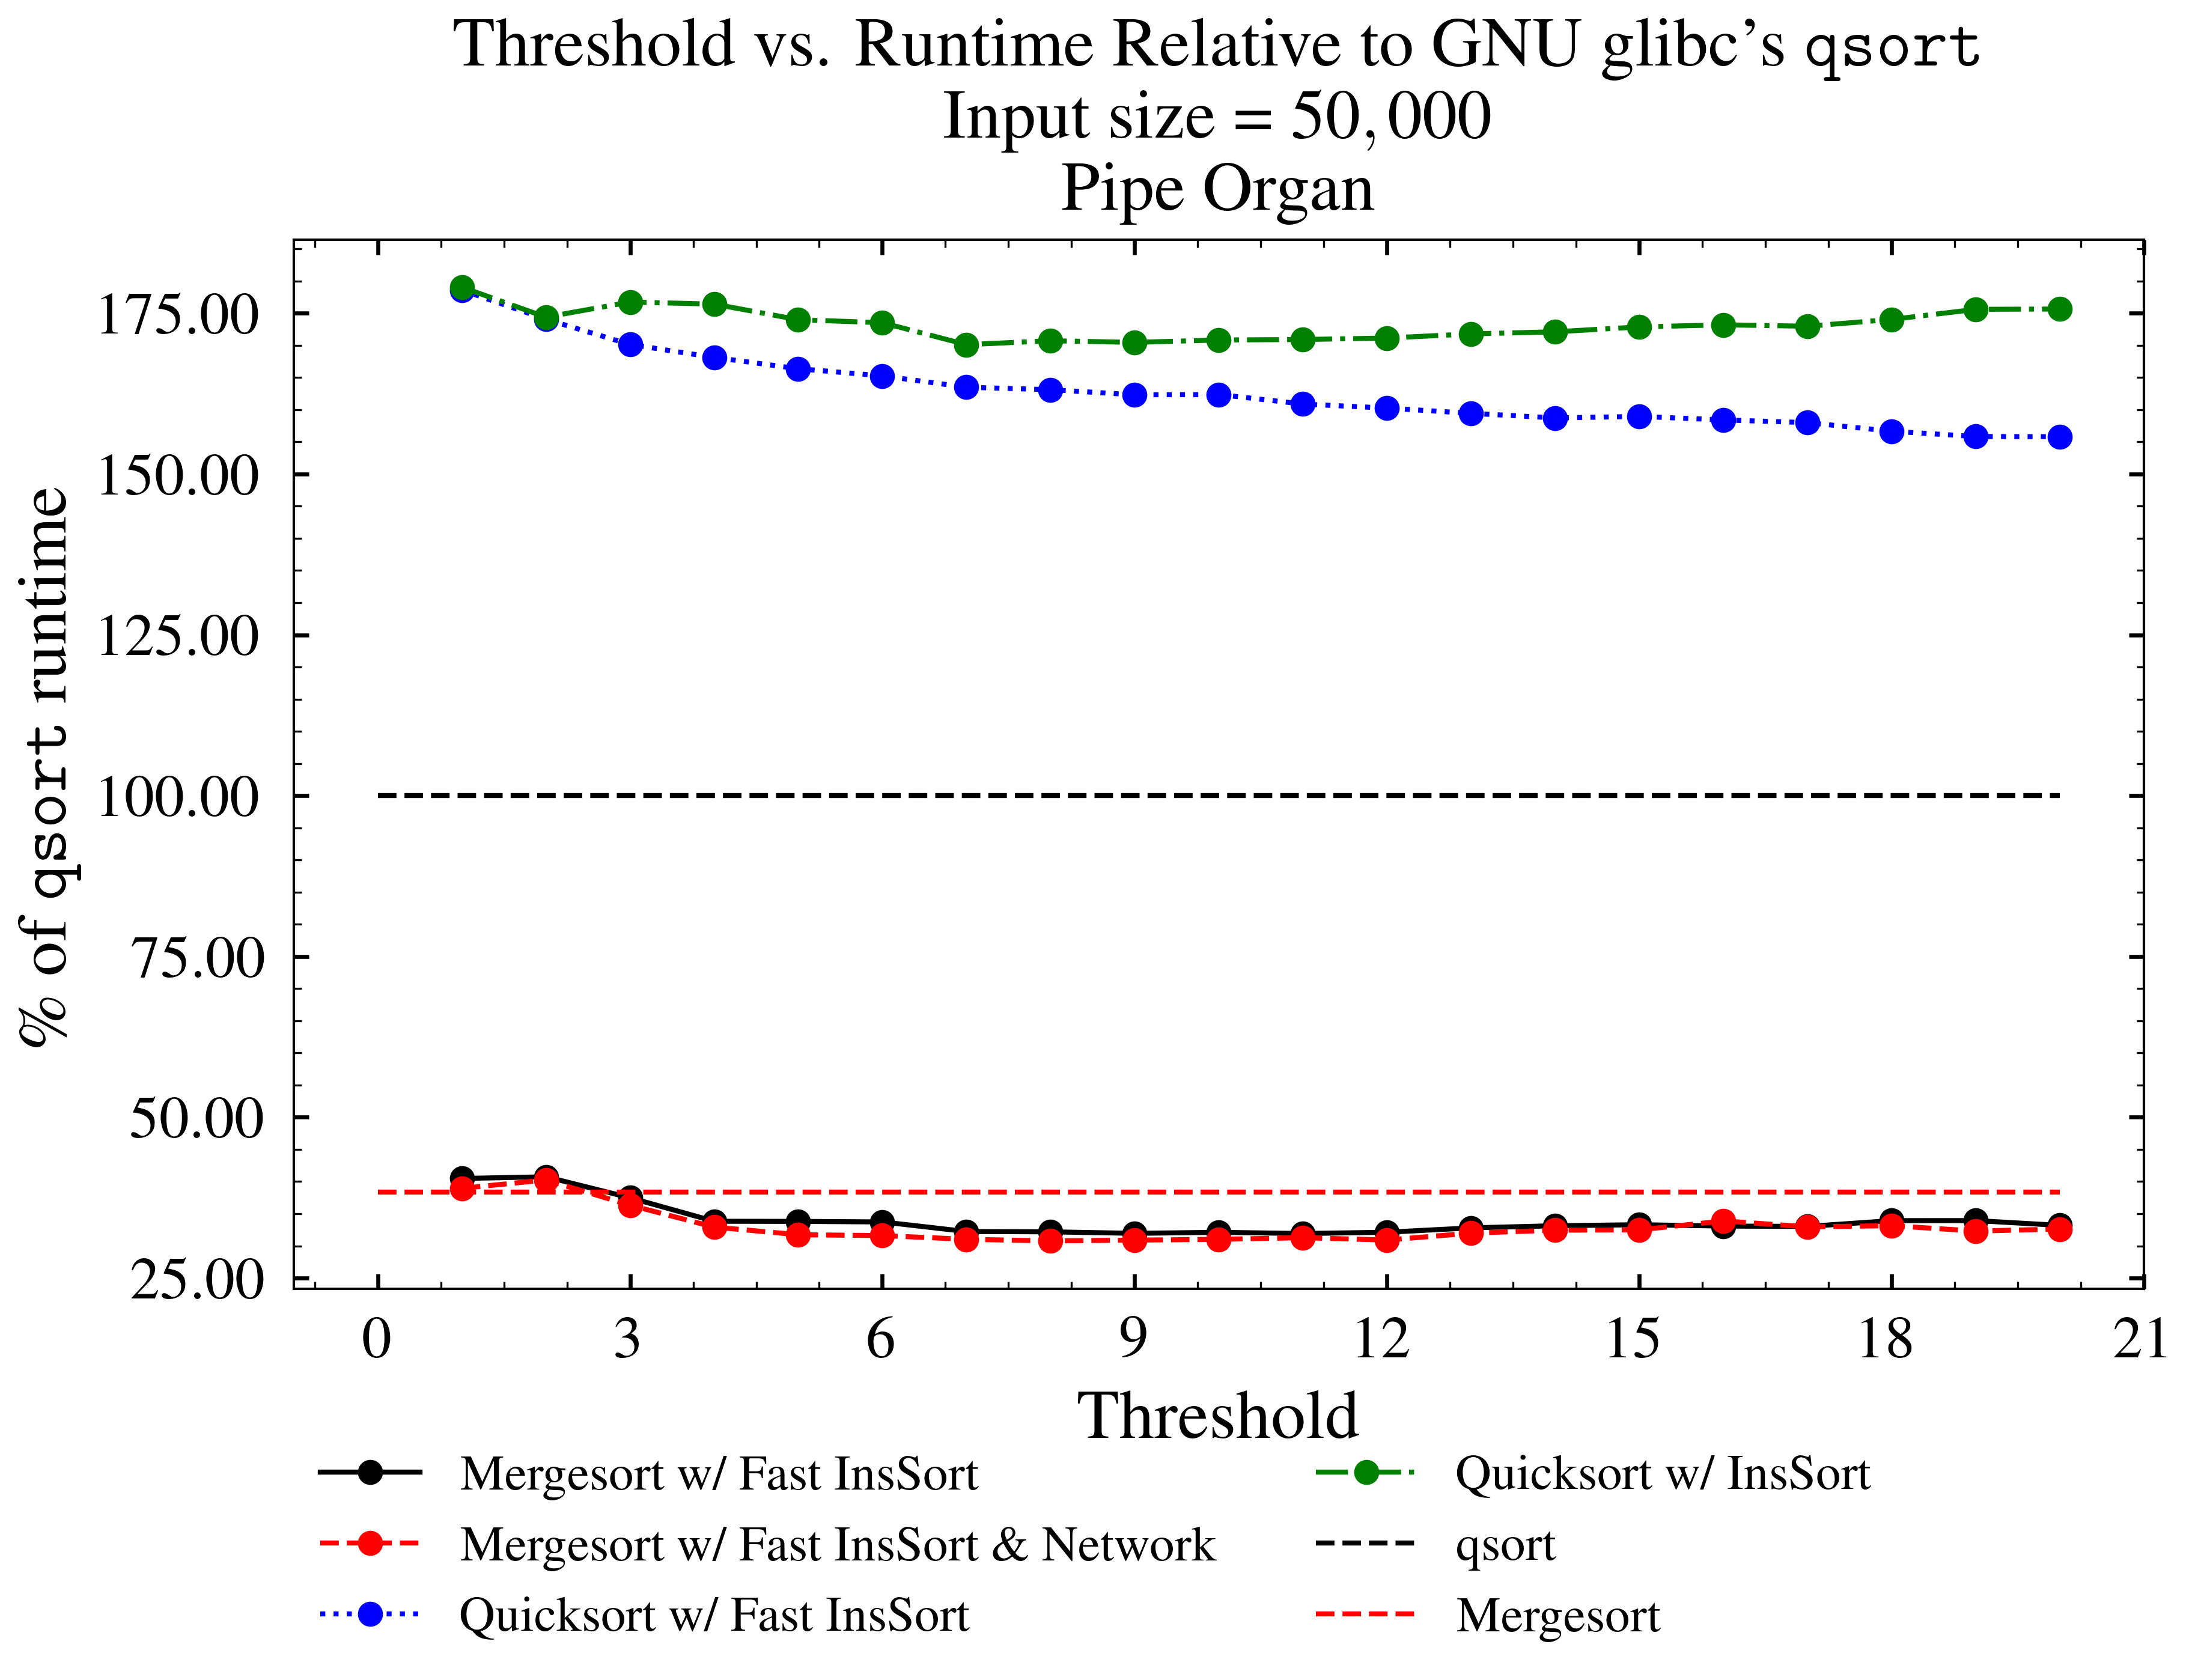
\includegraphics[width=\colwidth]{pipe_organ}}
					\caption{Runtime vs. Threshold on Pipe Organ Input Data}
					\label{fig:pipeorgan}
				\end{figure}
			\end{block}
		\end{column}

		\separatorcolumn

		\begin{column}{\colwidth}

			\vspace{10mm}

			\begin{block}{}
				To ensure the proposed algorithm is performant in a wide variety
				of hardware configurations, tests are repeated on various
				different platforms with differing CPU and memory setups. The best
				configurations are compared with each other to determine how well
				each algorithm generalizes across many platforms. Some platforms
				see little improvement with the additional hybridization of
				networking sorting, while others see significant performance
				gain. This indicates an area in need of further investigation.
				\begin{figure}[h]
					\centering
					\makebox[\colwidth]{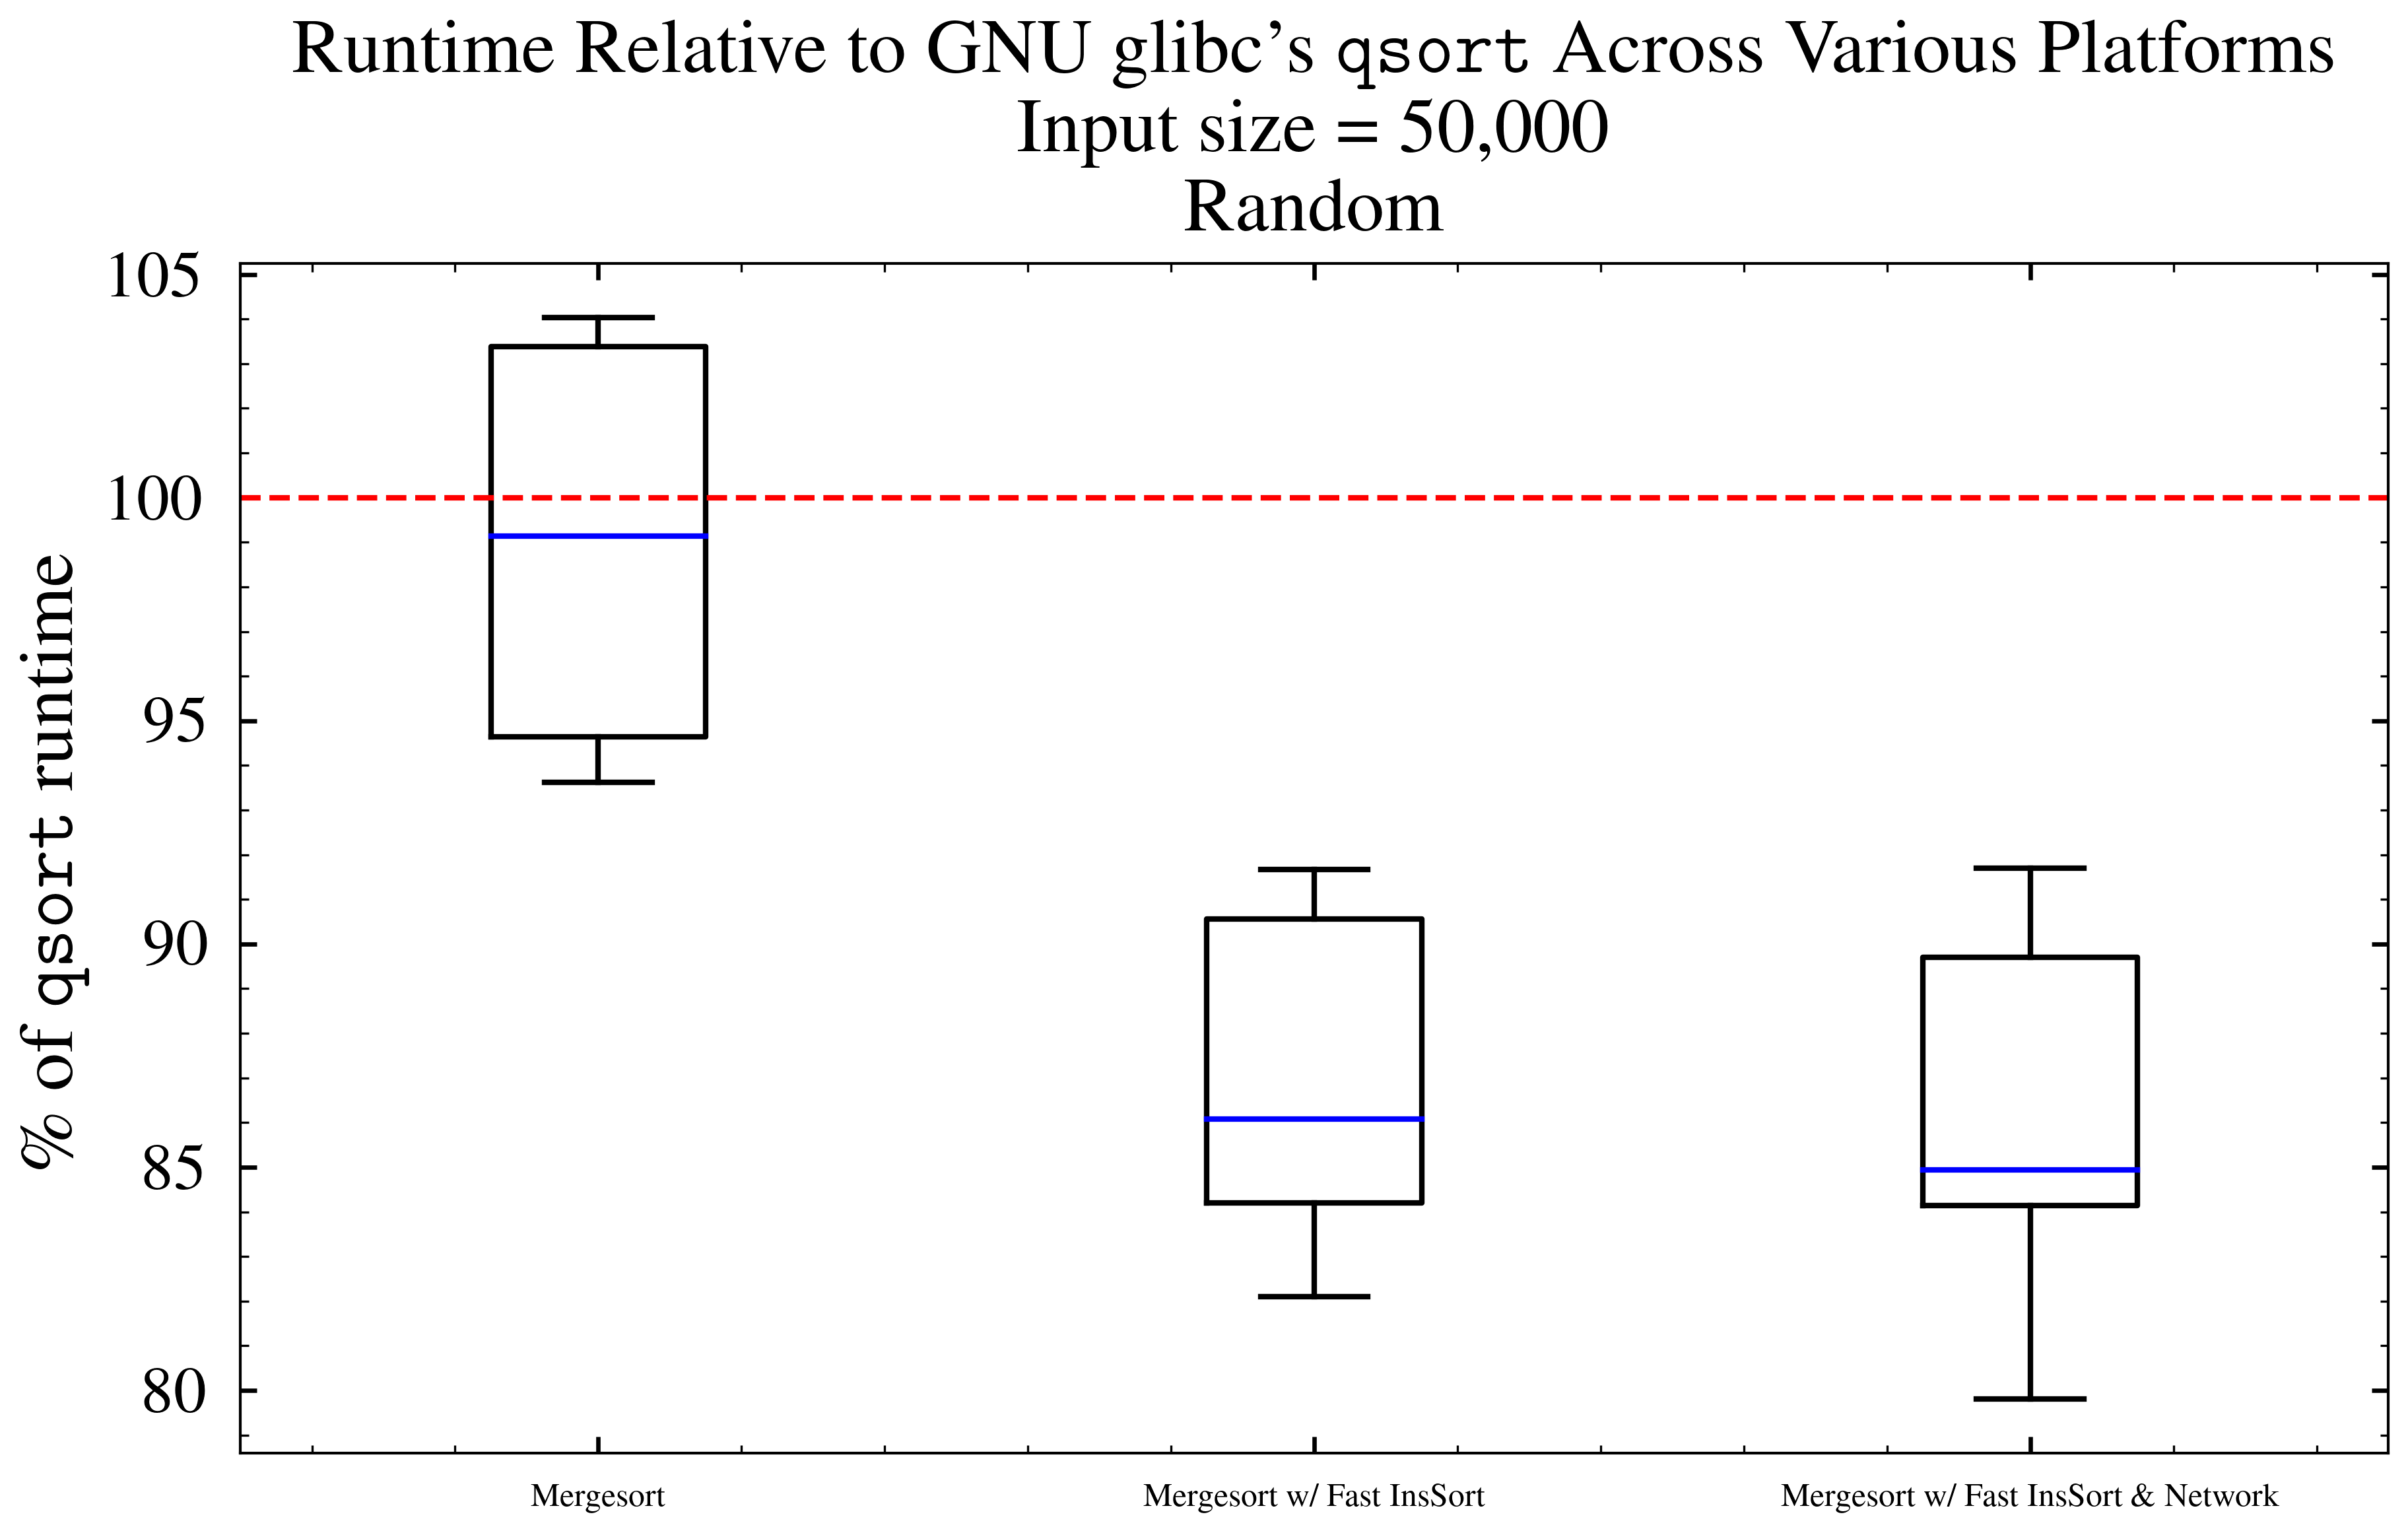
\includegraphics[width=\colwidth]{boxplots/4.gen}}
					\caption{Best Runtime By Method Across Various Platforms on Random Input Data}
					\label{fig:randomvariance}
				\end{figure}
				\begin{figure}[h]
					\centering
					\makebox[\colwidth]{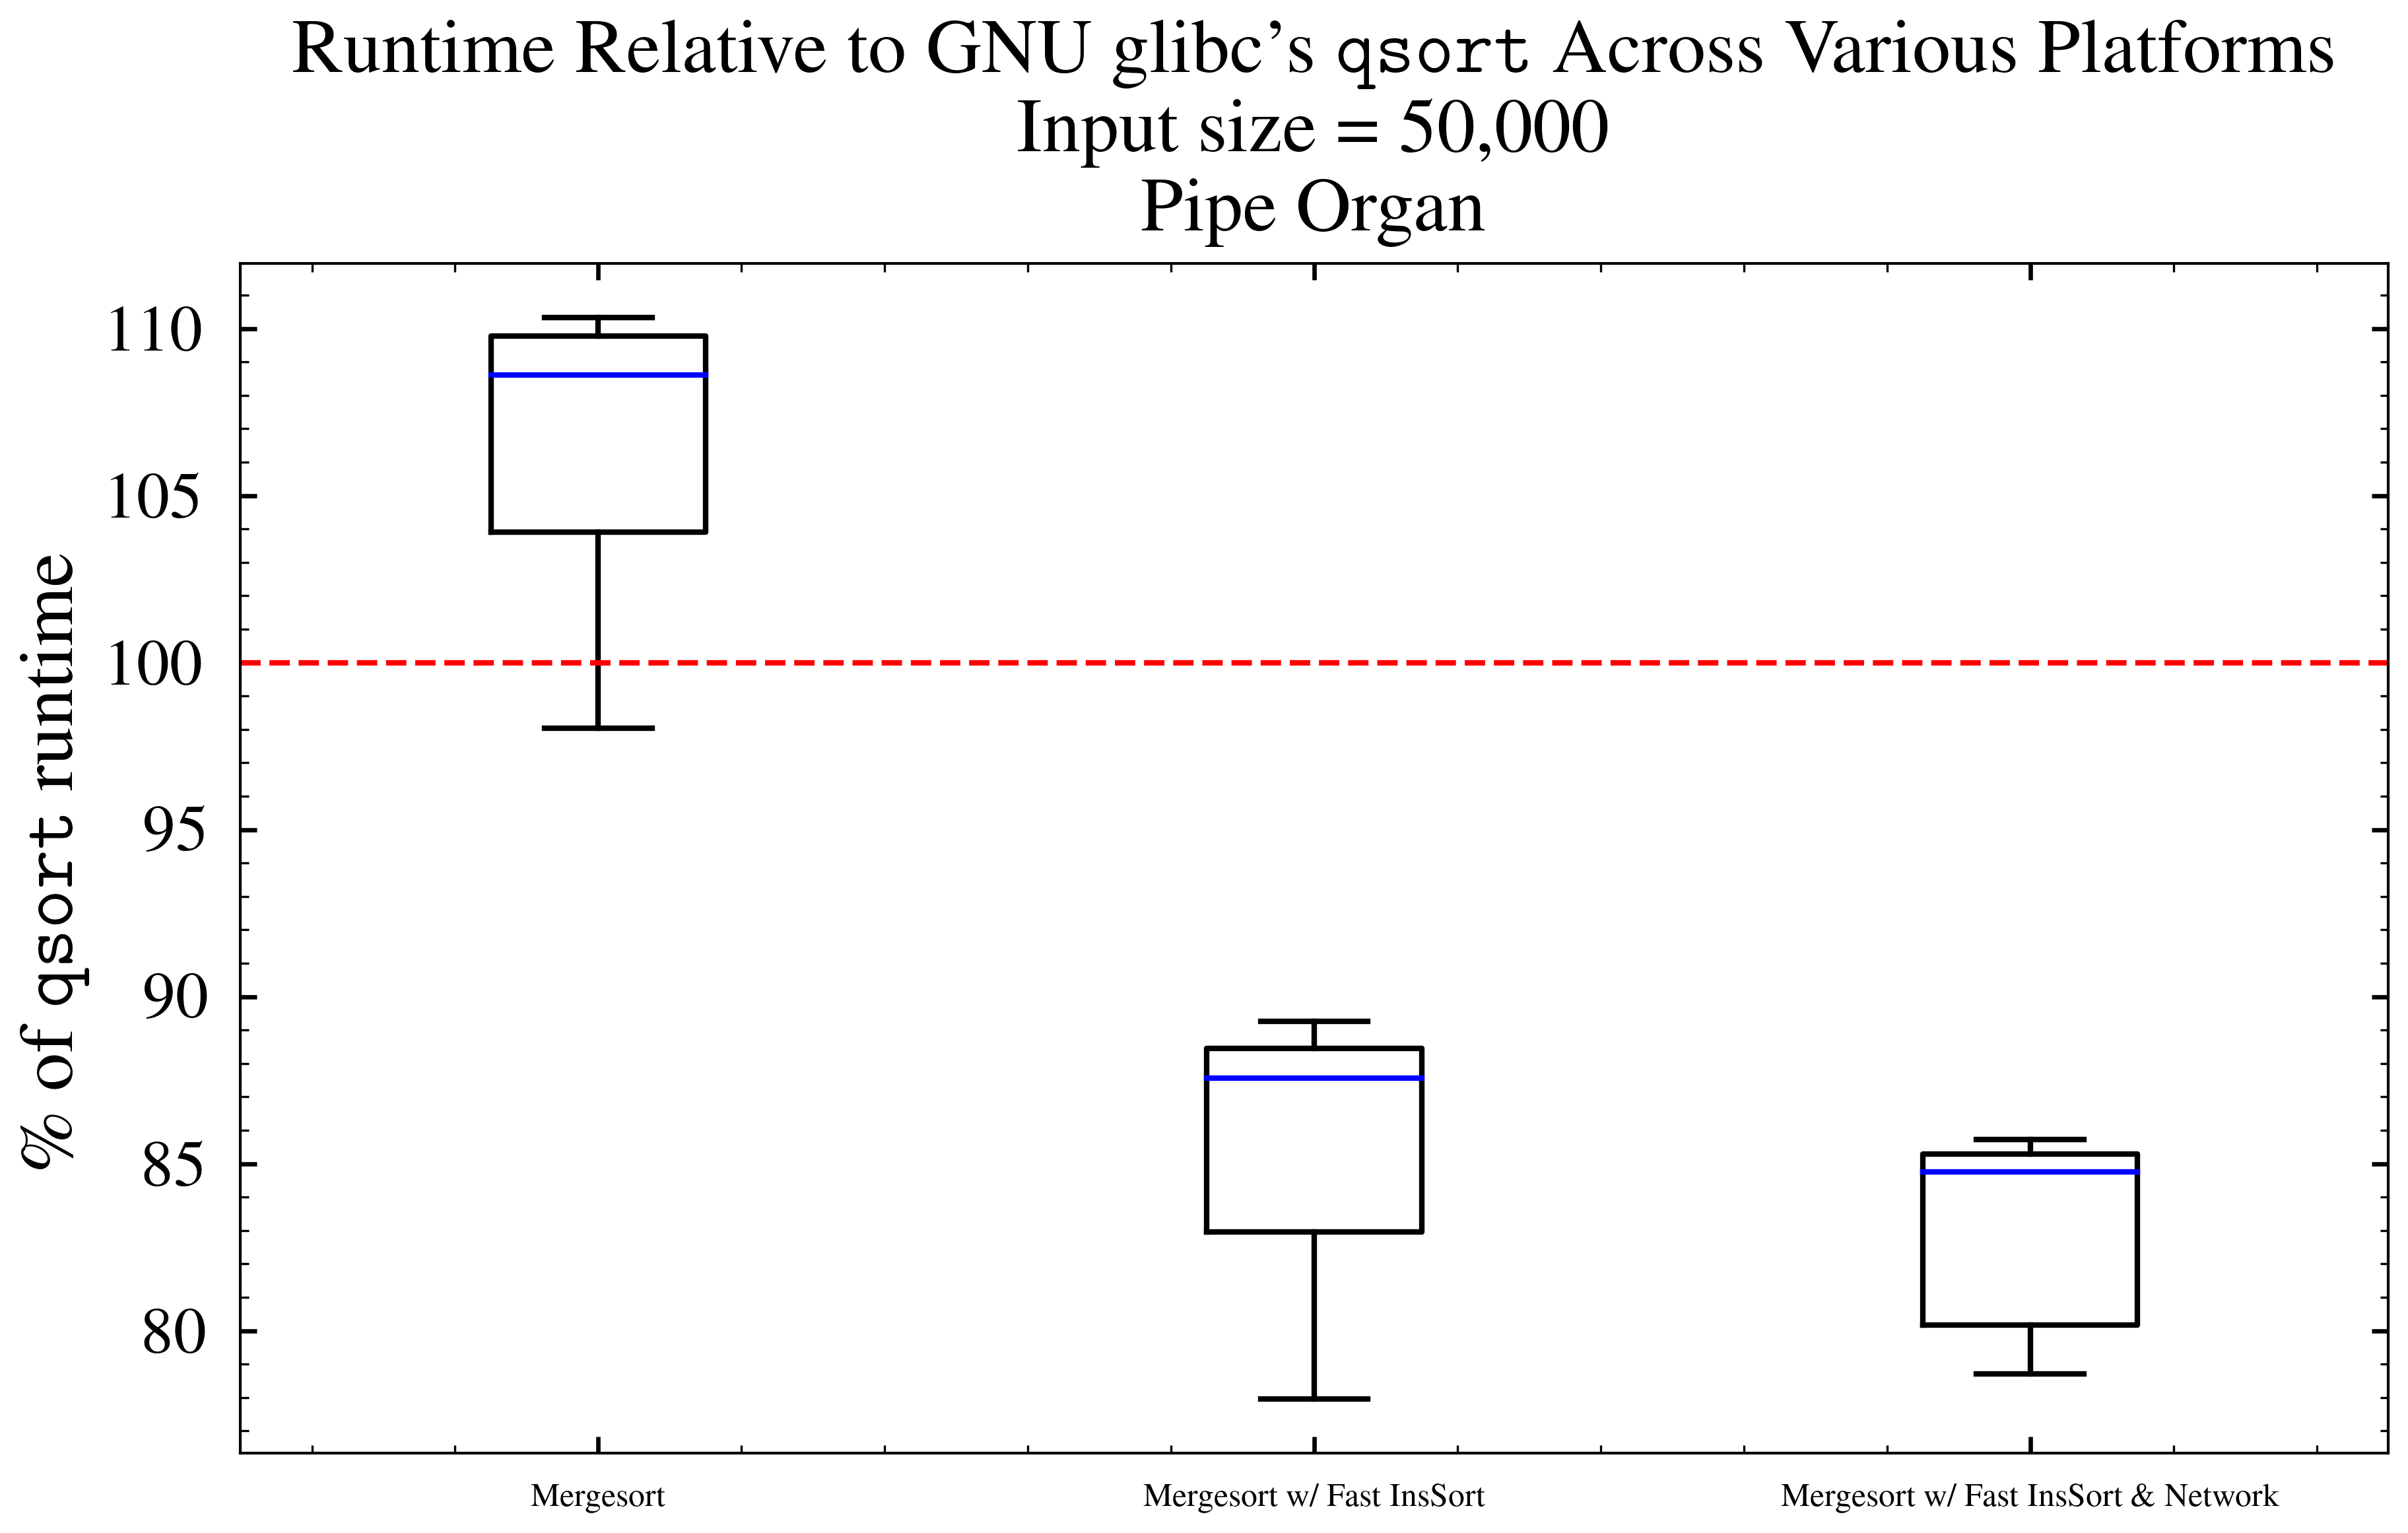
\includegraphics[width=\colwidth]{boxplots/0.gen}}
					\caption{Best Runtime By Method Across Various Platforms on Pipe Organ Input Data}
					\label{fig:pipeorganvariance}
				\end{figure}
			\end{block}

			\nocite{ARCC}
			\begin{block}{References}
				\footnotesize{\printbibliography}
			\end{block}
		\end{column}

		\separatorcolumn
	\end{columns}
\end{frame}

\end{document}
